\documentclass[10pt]{article}
\usepackage[margin=0.75in]{geometry}\usepackage{amsmath,amssymb,booktabs,graphicx,xurl,needspace}
\usepackage[colorlinks=true,urlcolor=blue]{hyperref}\setlength{\parindent}{0pt}\setlength{\parskip}{5pt}\emergencystretch=2em
\title{Certified structural properties of the curve catalogue}\author{Fixed-model classification and independent replay}\date{11 October 2026}
\begin{document}\maketitle
Native arithmetic and PARI agree on all 814 exact models. We certify 360 ordinary 2-volcano levels and retain bounds for 454. Among the 512 independent 192--252-bit sources, 219 are certified at the 2-surface and 65 have full rational 4-torsion. Original model identities and family/class labels are retained.
\section{Inventory and evidence}
The 277 $p=7$ route/conversion/control models are postselected; 25 higher-degree models are constructed controls. The 512 independent large sources retain their original model law, including full rational 2-torsion by construction. All retained models are ordinary. Counts describe these inventories, with no uniform-class density or sampling-error interpretation. Field sizes are $7^6$ (17 bits) and 192--252 bits, in degrees 6, 10 and 14. Selected subgroups and generators remain unspecified.
\begin{figure}[ht]\centering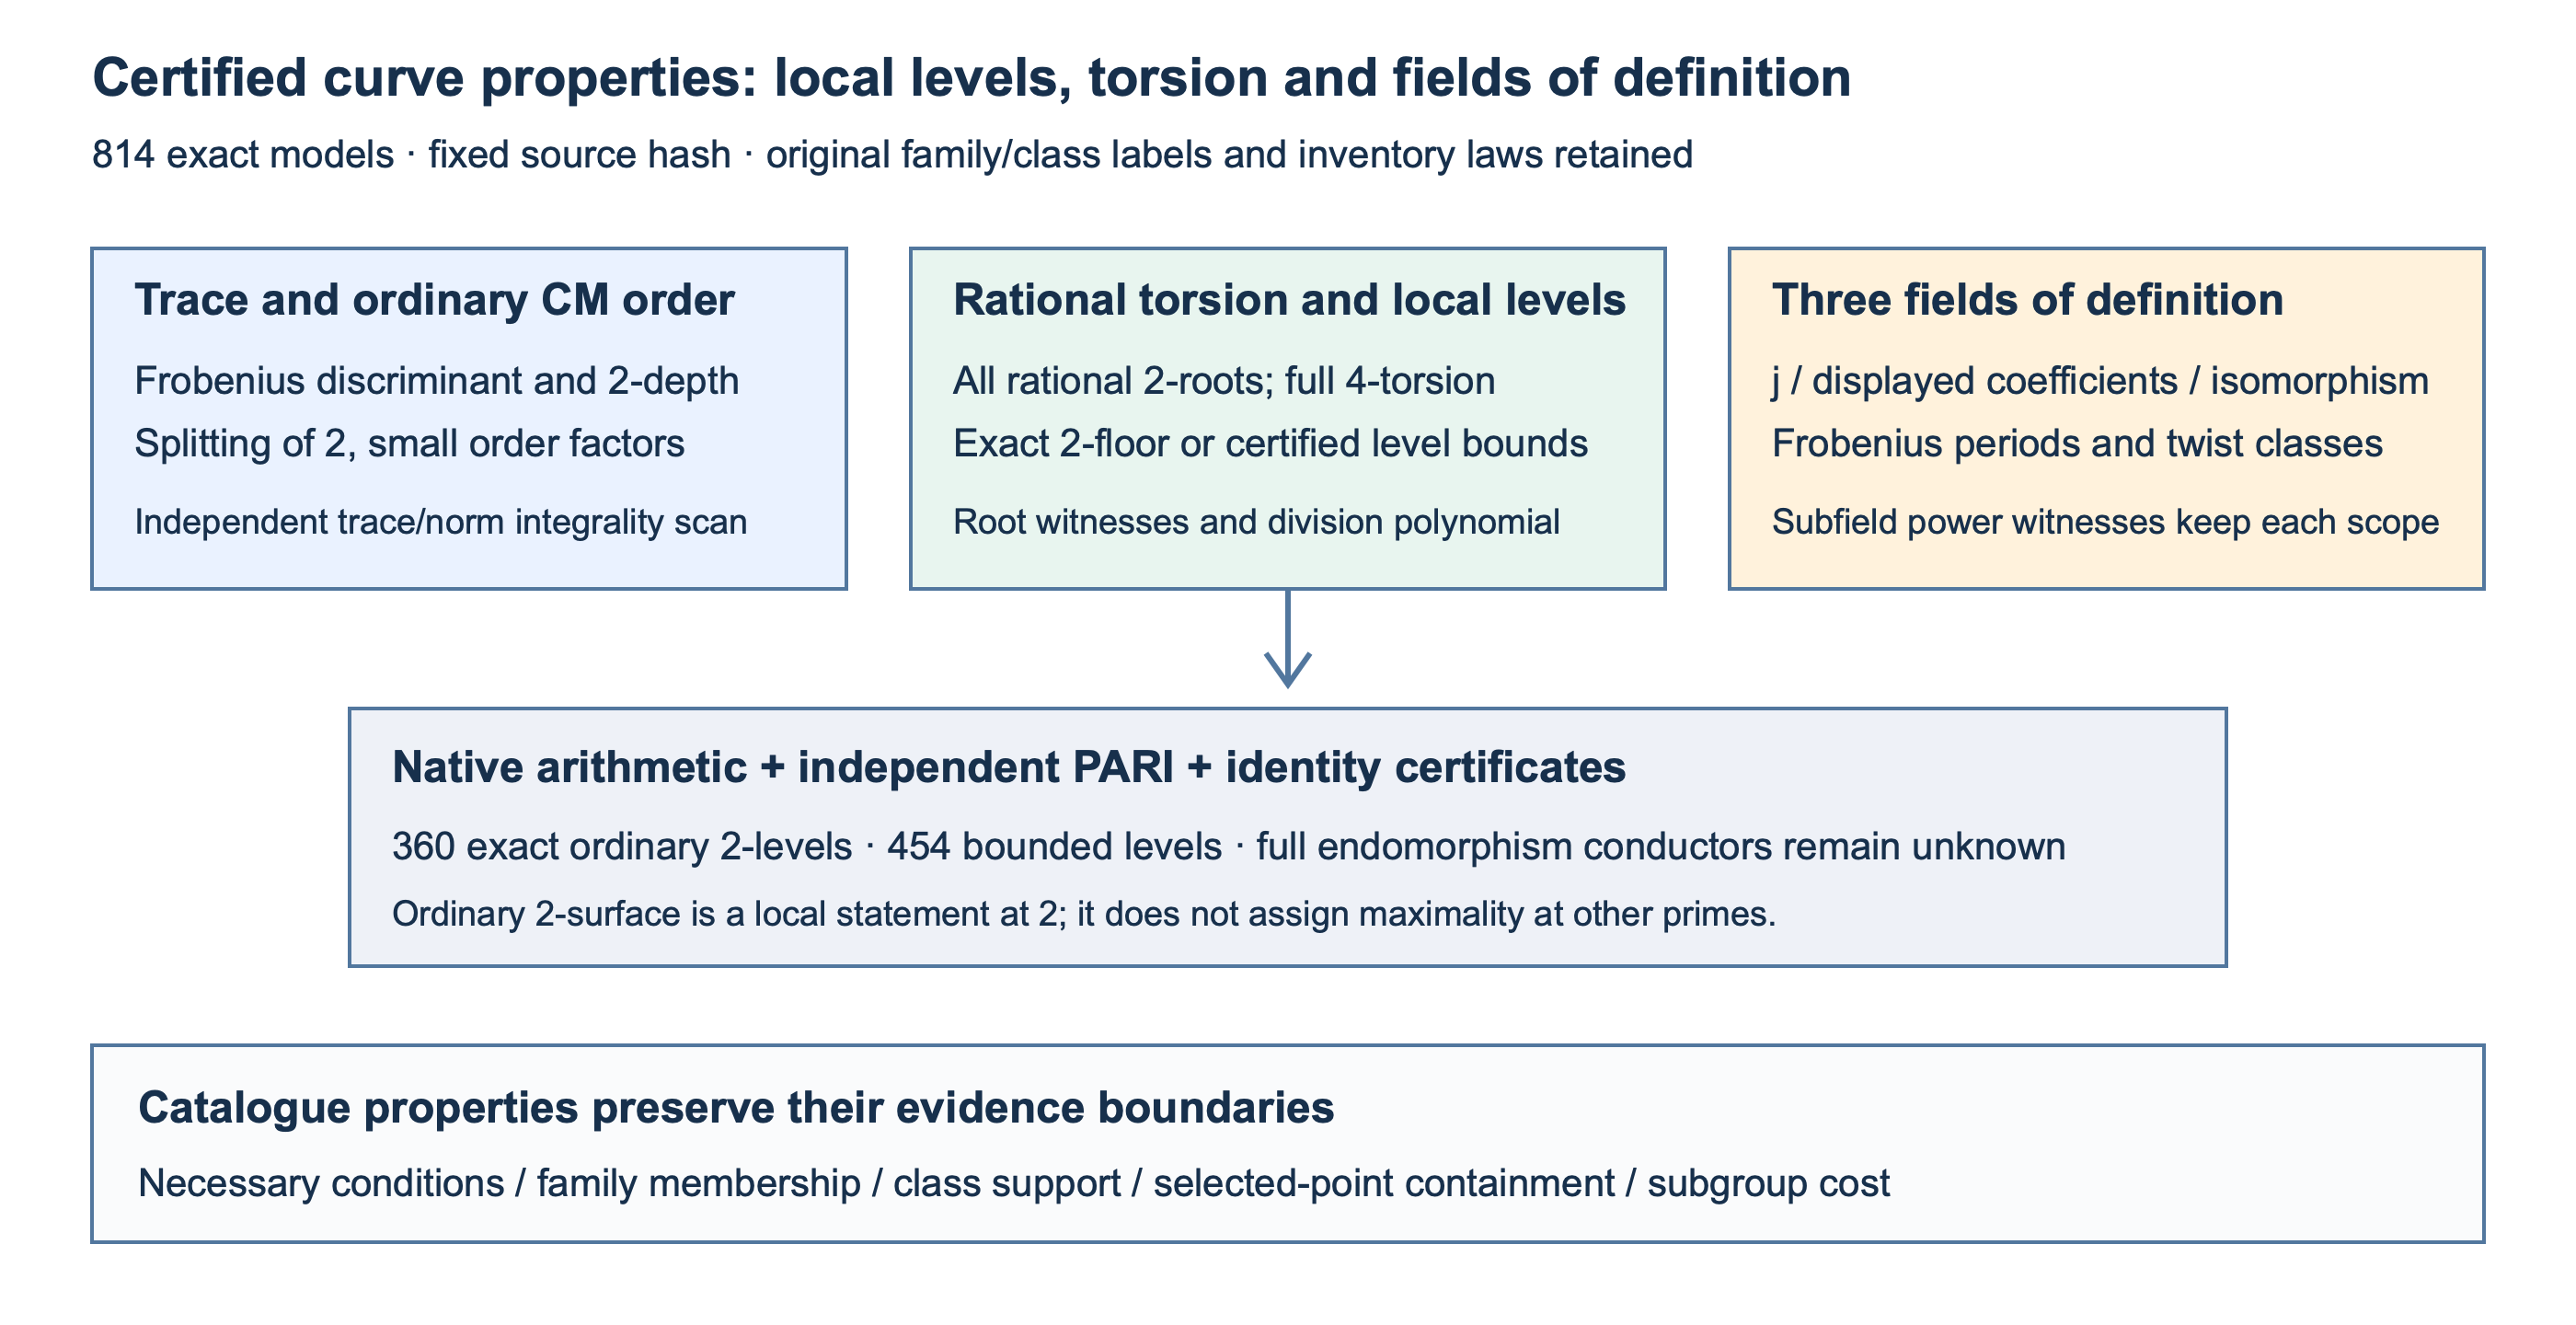
\includegraphics[width=\linewidth]{property_pipeline.png}\caption{Independent structural properties feed the existing catalogue without promoting a necessary filter to family membership.}\end{figure}
\begin{center}\small \begin{tabular}{lrrrrrr}\toprule Inventory & Models & Full 2 & Full 4 & Exact level & Bounded & Proper iso\\\midrule
p7 replay/control & 277 & 200 & 52 & 116 & 161 & 3\\
Higher-degree controls & 25 & 0 & 0 & 25 & 0 & 0\\
Independent large sources & 512 & 512 & 65 & 219 & 293 & 0\\
\bottomrule\end{tabular}
\end{center}
\begin{figure}[ht]\centering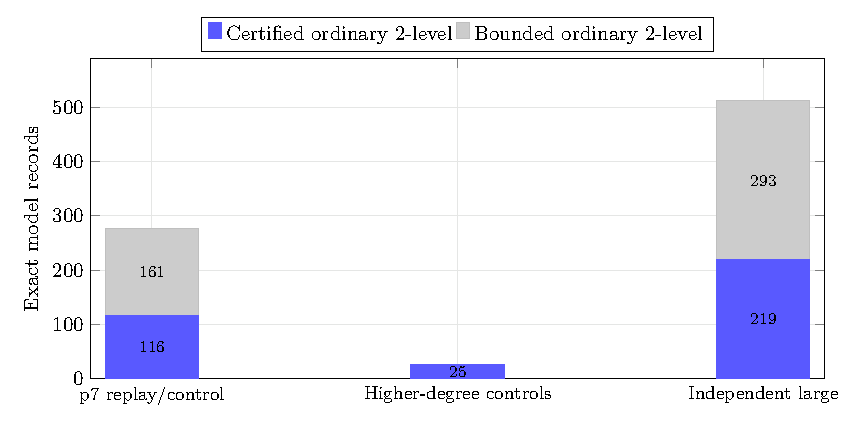
\includegraphics[width=0.92\linewidth]{level_coverage.pdf}\caption{Exact and bounded ordinary 2-levels in each frozen model cohort. Units are model records; cohort input laws differ.}\end{figure}
\section{Local conductor data without odd factorization}
For an ordinary trace write $\Delta=t^2-4Q=2^s u<0$ with $u$ odd. Fundamental-discriminant classification gives
\[
v_2(D_K)=\begin{cases}3&s\text{ odd},\\0&s\text{ even and }u\equiv1\pmod4,\\2&s\text{ even and }u\equiv3\pmod4.\end{cases}
\qquad v_2(f_\pi)=\frac{s-v_2(D_K)}2.
\]
Odd squares are one modulo eight, so the odd fundamental-discriminant residue determines split/inert behavior of two; a positive two-valuation is ramified. Full $D_K$ and the odd conductor remain uncomputed.

PARI independently searches integral $(\pi-a)/2^k$, whose trace and norm must both be integers:
\[
\frac{t-2a}{2^k},\qquad \frac{Q-at+a^2}{2^{2k}}.
\]
For even $t$ there are two possible $a$ residues modulo $2^k$; odd $t$ permits no positive $k$. In a maximal-order basis $\pi=A+f_\pi\omega$, the largest admissible denominator is exactly $v_2(f_\pi)$. This method checks every ordinary model, with a full-discriminant cross-check on the small discriminants.
\section{Torsion certifies ordinary 2-levels}
\textbf{Proposition.} Let $E/\mathbb F_Q$ be ordinary in odd characteristic and let $s=v_2(f_\pi)$. Exactly one rational nonidentity 2-point implies $v_2(f_E)=s$, the ordinary 2-volcano floor. Full rational 2-torsion implies $v_2(f_E)\le s-1$; full rational 4-torsion implies $v_2(f_E)\le s-2$. A collapsed bound certifies the local level.

\textbf{Proof.} In a basis $1,\omega$ of $\operatorname{End}(E)$, write $\pi=a+b\omega$. The order index is $f_\pi=f_E|b|$. Full rational $E[2]$ is equivalent to $\pi-1\in2\operatorname{End}(E)$: an endomorphism killing $E[2]$ factors through the separable map $[2]$. If $b$ is even, the odd norm $Q$ forces $a$ odd, giving this divisibility. Absence of full rational 2-torsion therefore forces $b$ odd and the floor equality. Full rational $E[4]$ similarly implies divisibility by four and the second bound.\hfill$\square$

The native checker validates all rational 2-roots and uses their differences and the square class of $-1$ to certify full 4-torsion. PARI independently uses the sextic factor of the degree-four division polynomial and the square classes of its $y$ coordinates. Whole endomorphism conductors remain unknown; a 2-surface statement does not assert maximality at other primes.
\section{Three fields of definition}
The least Frobenius period of $j$ determines its degree; the joint period of $a,b$ determines the displayed model's degree. A $K$-isomorphic model can have a different minimum degree.

For generic $j$, set $a_0=3j/(1728-j)$ and $b_0=2j/(1728-j)$. The twist parameter is $D=3b/(2a)$, with $a=D^2a_0$ and $b=D^3b_0$. At $j=0$ use $b$ modulo sixth powers, and at $j=1728$ use $a$ modulo fourth powers.

For a candidate $\mathbb F_{p^d}$, put $M=p^n-1$, $m=p^d-1$ and $h=\gcd(\text{twist order},M/m)$. The image subgroup $\mathbb F_{p^d}^{*}(K^{*})^{\text{twist order}}$ is generated by the $h$-th power of a cyclic generator. Thus the twist parameter lies in it exactly when its $M/h$ power is one. Each row retains all candidate power witnesses, including rejected smaller fields.

Four $p=7$ records have $j$ degree three. Three have a $K$-isomorphic model over $\mathbb F_{7^3}$, and one requires $\mathbb F_{7^6}$. Only one already displays coefficients over $\mathbb F_{7^3}$:
\begin{center}\begin{tabular}{lrrr}\toprule Exact model slug & $j$ & Coefficients & Isomorphic model\\\midrule
\texttt{icv1-fp3k6-tm110-5f712c89} &3&6&3\\
\texttt{icv1-fp3k6-t202-39e02f24} &3&6&6\\\bottomrule\end{tabular}\end{center}
These are model-definition properties. Selected-point and subgroup containment remain unspecified.
\section{Certificates and verification}
Thirteen portable identity certificates cover the cubic discriminant, cleared normalized-$j$ and twist coefficients, translated Frobenius norm and eight unit-group index degrees. Each passes 64 saved and 128 fresh evaluations; native expansion additionally checks exact integer coefficients. IDs and expression trees are in \texttt{identity\_certificates.json}; the formal-proof pointer remains null.

Native arithmetic and PARI agree on all 814 property rows. Audit run 2 completes under its 300-second cap with empty stderr. The initial stack-setting initialization failure, its zero-row receipt and executed sources are retained. Point counts are reused from the independently verified parent records. Ten $p=7$ records have 13-smooth ambient order; residual cofactors are unclassified, and selected-subgroup costs are unmeasured.

The property browser is a sidecar. The earlier catalogue study and two-branch evidence remain sealed, and numerical IC ratio/census graphs retain their values: this round adds structural classification rather than a new paired timing measurement. Reproduction, source hashes, identity IDs and raw arithmetic evidence are linked in the Markdown report and validation record.
\section{Sources}
\href{https://math.mit.edu/classes/18.783/2023/LectureNotes13.pdf}{Sutherland: ordinary/supersingular curves and endomorphism orders}.\par
\href{https://math.mit.edu/classes/18.783/2023/LectureNotes22.pdf}{Sutherland: isogeny volcanoes}.\par
\href{https://pari.math.u-bordeaux.fr/dochtml/html-stable/Arithmetic_functions.html}{PARI: arithmetic and fundamental discriminants}.\par
\href{https://pari.math.u-bordeaux.fr/dochtml/html/Polynomials_and_power_series.html}{PARI: finite-field polynomial roots}.\par
\href{https://github.com/aburan28/crypto/blob/862f35365af35cdbc29a2cd9b6ab63037afb668c/research/iso1_weak_classes_20261007/two_branch_20261009/REPORT.md}{Parent two-branch theorem and frozen model evidence}.
\end{document}
